\documentclass[12pt,a4paper,smallheadings,cleardoubleplain,DIV8]{scrbook}
\usepackage{pyblio,graphicx,mdwlist}
%\includeonly{td-rg3}
% add font styles  like: ,galliard,gillsans, if you like
\hyphenation{data-base}
%\rcsInfo $Id$
\begin{document}
\frontmatter
\title{Pybliographer\\ User's Reference Guide}
\author{Fr�d�ric Gobry and Peter Schulte-Stracke}
\maketitle{}
\mainmatter
\pagestyle{headings}
% \begin{abstract}This manual gives an introduction and reference for
%   the use of Pybliographer version 2.
% \end{abstract}

%%% ad interim 
\newcommand{\myrulewidth}{.8pt}
\newenvironment{dnote}{\par\medskip\centerline{\textbf{Note}}\vspace{-7pt}
\noindent\rule{\textwidth}{\myrulewidth}\begin{itemize}}
{\end{itemize}\rule{\textwidth}{\myrulewidth}\\[2pt]\noindent}

\newenvironment{dtask}{\par\medskip\centerline{\textbf{Task}}\vspace{-7pt}
\noindent\rule{\textwidth}{\myrulewidth}\begin{itemize}}
{\end{itemize}\rule{\textwidth}{\myrulewidth}\\[2pt]\noindent}

\newenvironment{drequ}{\par\medskip\centerline{\textbf{Requirements}}
\vspace{-7pt}\noindent\rule{\textwidth}{\myrulewidth}\begin{itemize}}
{\end{itemize}\rule{\textwidth}{\myrulewidth}\\[2pt]\noindent}

\tableofcontents
\reversemarginpar

% Part 1 -- Introduction
\part{Introduction}

\chapter[Introduction]{A Primer for Pybliographer}
\label{cha:rgintro}


This chapter provides an introduction to \Pyb\ for new users.
If you are already familiar with \Pyb, you can skip this chapter.


\section{What Is Pybliographer, and Why Should I Use It? }
\label{sec:whyuse}




Pybliographer provides Reference manager services to create, load,
modify, list, read, transport, and copy description of ressources like
books, articles, and electronic documents, including derivative and
private information.

[[Many restrictions inherent in the  BibTeX database format used by
earlier versions of this program are removed or relaxed in this
version. 

This version continues to support \BibTeX\ databases to assist you in
converting to the new database structure. [XXX Subsequent releases,
however, might not support these features, so we strongly recommend
conversion to the exclusive use of the new database structure.

Support for using \BibTeX\ as an import and export format only,
however, is planned for the foreseeable future.] 
]]



\paragraph{A first example}

\label{sec:first-example}

Let's consider a simple situation first.  During a talk with a friend,
you suddenly remember a paper that you read a while ago.  Back home,
you look it up in your Pybliographer Database:

In the Search Window (Fig. \ref{fig:searchx1}) you enter the author name and
a word from the title (other approaches are possible and are discussed
in section XXX):

\begin{figure}[htbp]
  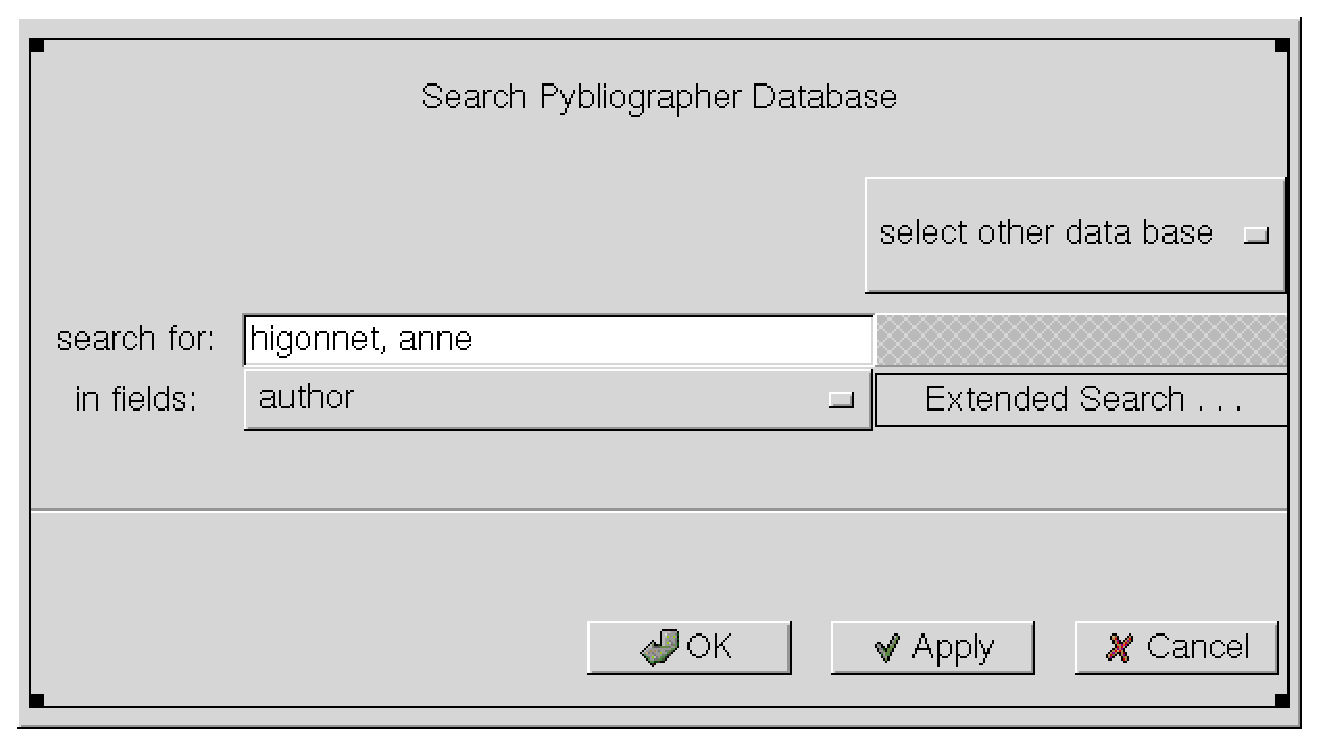
\includegraphics[width=.6\textwidth,bb=0 0 617 342]{pics/searchx1.eps}
  \caption{Search window with example search terms entered.}
  \label{fig:searchx1}
\end{figure}


The system replies by displaying the list of one item found, and also
the first and only item in a subwindow (Fig. \ref{fig:searchx2})

\begin{figure}[h]
  
  \caption{Display of example search results}
  \label{fig:searchx2}
\end{figure}

You decide to e-mail the citation to your friend. You can easily
insert it into the e-mail with the standard \textit{drag-and-drop}
mechanism that Pybliographer supports. The format of the citation is
easily selected and changed (XXX).

Perhaps you should try and look for some other references in this area
when your are in the library again? Let's attach a note to the item,
so as to be reminded of it when you visit the library the next time: 

\begin{figure}[h]
  
  \caption{Adding an action note}
  \label{fig:searchx3}
\end{figure}


\paragraph{Writing an article}

\label{sec:writing-an-article}

It's only a short note this time, so we don't need much preparation. A
review say, the book lays on your table, a couple of notes, the editor
is started. You didn't enter the book into your database yet, so you
start with querying your national library (see Fig.~\ref{fig:searchx4}
). This has the useful side effect of telling you whether the author
in question has already published something (no need to put your foot
in it).

\begin{figure}[h]
  
  \caption{Looking up an author in an external database}
  \label{fig:searchx4}
\end{figure}

Whenever you look something up in this way in an \textit{external
  databaese}, as opposed to the Pybliographer database, the result of
your query will be captured in an internal list, it is then available
for further processing, but not yet entered into the Pybliographer
database. The reason for this is, that it may be too much work for the
moment -- and it is work that must be done diligently -- to check-in
and adapt each an every item that a database query might deliver. (See
the next chapter, in particular ... for more information on this.)
But in this case, there are but two items, which are easily added.

If the information comes, as it is here presumably the case, from a
Z39.50 connected and MARC serving database, there is usually little to
do at this stage. One point, however, remains to do: the new entries
must be correctly categorised, lest our fine arrangement goes to
pieces. If we are content with the standard folder mechanism, it
should suffice to travers the folder hierarchy until the right leave
is found, then to drop the item(s).

\begin{figure}[h]
  
  \caption{Dragging an item into a folder}
  \label{fig:searchx5}
\end{figure}
 
To commence the article, you drag the corresponding item on the editor
window and drop it there: the formatted bibliographical reference is
inserted and easily edited by you for publication.

You follow this first paragraph by your observations, occasionally
consulting your paper notes perhaps. Oh, and this paragraph on page
123 you would like to quote, but first you enter it in Pybliographer's
quotation storage. (XXX) A new editor window appears and already knows
the item from which you want to enter the text. It first asks you for
the page number, so you cannot forget it, and then lets you enter and
edit the text. 

\begin{figure}[h]
  
  \caption{Entering a quotation}
  \label{fig:searchx6}
\end{figure}

By simply dragging the quote into the editor window you not only get
the text, but the citation as well. You decide to use only a portion
of the full quote, so you delete a portion of it. Then you want to add
another voice, whatever was his name \dots\ You decide to open the
author list and position it at the approximate name.

\begin{figure}[h]
  
  \caption{Displaying the author list}
  \label{fig:searchx7}
\end{figure}

You select and open the right entry (let's assume this), and
look down the list until you find the wanted entry. From the detail
view of this entry you could again choose a quote, but then you
decide otherwise, and simply cite this article instead, you already
guess, how to do it.

\begin{figure}[h]
  
  \caption{Citing an item}
  \label{fig:searchx9}
\end{figure}

Let's stay for a moment yet with the detil view: the article had been
quoted, you remember, and selecting the references view lets you find
this article as well. A sentence from here would fit in much better
with you review, wouldn't it? 

\begin{figure}[h]
  
  \caption{Excerpt -- sections and quotes}
  \label{fig:searchxa}
\end{figure}

When you are finished with your work, Pybliographer does the
bibliography for you, simply select Format/references from the
Menu. You need to specify a stylesheet, and some other options, and
then you can lay back and relax.

\begin{figure}[h]
  
  \caption{Dialogue Formatting options}
  \label{fig:dlformat1}
\end{figure}



%%% Local Variables: 
%%% mode: latex
%%% TeX-master: "td-td2"
%%% End: 


\chapter{Pybliographer Concepts}
\label{cha:rgconc}

This chapter summarises some basic concepts that you need to
understand before you can use \Pyb.
It briefly describes:
\begin{itemize}
\item What bibliographic items are and how they are described
\item What basic data types are used 
\item How the data is stored and processed
\item How \Pyb\ can help you storing and editing bibliographic
  resources and using them in you work
\end{itemize}

% \chapter{Working with Pybliographer}
% \label{cha:rg2}

% \newcommand{\Pyb}{Pybliographer{}}

% When you work with \Pyb, you will do so most often through one of the
% following windows:

% \begin{itemize}
% \item The Search Window
% \item The Folder Window
% \item The List Window
% \item The Detail Window
% \end{itemize}

% Often you will start with the Search Window. Enter a search term and
% start a search.  (See \ref{fig:searchx1}) The same window allows you to
% query another (possibly remote) database, and to formulate more
% complicated queries.

% Alternatively, you can open a predefined collection of records, a
% \textit{folder} or \textit{list}.  The \textit{Folder Window} allows
% you to select from all the folders and lists available. It can also be
% shown permanently as a left sidebar. Click on the small triangle to
% the left of each entry to open or close a folder in this display. Click
% on the name to display its contents in the list window.

% A list is simply a folder that is found under the label Lists at the
% beginnign of the folder display; together with the entries Marked,
% \dots

% Whatever your way, you will sooner or later see a \textit{List
%   Window}. It shows your current \textit{selection}. Usually records
% are ordered by name of first author and are displayed in a condensed
% format. Those are options that are easily set and changed; it is
% possible to tie thses settings to a particular list; think os a
% shopping list for you rnext visit to the library, that you might like
% always sorted by location.
  
% To inspect an item it is often sufficient to point with the mouse to
% it, and have a tooltip like preview window appear. It allows at the
% same time to concisely inspect  the entry and also to preview it in a
% typical format (both can be configured, of course).  Alternatively,
% you may open the deatil view (inspector) for an item. It presents you
% with a lot of information in a notebook widget. 







%%% Local Variables: 
%%% mode: latex
%%% TeX-master: "td-td2"
%%% End: 


\chapter{Preparing to Use Pybliographer}
\label{cha:rgprep}

This chapter discusses how to install and configure \Pyb.


It  describes how to do the following:

\begin{enumerate}
\item Install \Pyb.
\item Set up the required database structure
  \begin{itemize}
  \item Determine which databases to use
  \item Define the directory structure or access path
  \item Define additional data that you might need
  \end{itemize}
\item Set up \Pyb\ for easier operation
\item Load needed data
\item Write local processing routines
\end{enumerate}


% \chapter{Describing ressources}
% \label{cha:rgdesc}


% \section{General considerations}
% \label{sec:descgen}


% When describing ressources of any kind, we encounter some problems
% again and again. 

% The first has to do with the question which information to use; more
% specifically where to look for the information.

% To reduce the variation and confusion when describing ressources, there
% are certain established principles, among others:

% \begin{itemize}
  
% \item Use the original text, if possible. This principle avoids e.g.,
%   the confusion arising from giving a place of publication that is
%   \textit{K�ln, C�ln, Keulen, Cologne}, depending upon time and place
%   of cataloguing. 
% \item Use special normalised forms to account for the needs of users
%   that might not know the original form, but do not replace the
%   original form (for important pieces of information), but give both
%   of them.
% \item Prefer the information as it is found on the title page (and
%   some comparable places).  At least indicate information that does
%   not come from the standard places by putting it into brackets [].
% \item Distinguish the various classes of information, in particular do
%   not confound formal and material description, nor bibliogrpahic
%   description and annotations etc. although the software supports it
%   both. It much simplifies life to keep these purposes apart.
% \end{itemize}


% \section{Persons}
% \label{sec:rgpersons}




%%% Local Variables: 
%%% mode: latex
%%% TeX-master: "td-td2"
%%% End: 


\chapter{Entering Data}
\label{cha:rgnew}

This chapter discusses how you enter new data into the \Pyb\ database.
It describes:
\begin{itemize}
\item Sources and classes of bibliographic data
\item An example of creating a new record
\item Editing (modifying) data 
\end{itemize}





%%% Local Variables: 
%%% mode: latex
%%% TeX-master: "td-td2"
%%% End: 


\chapter{Searching and Selecting}
\label{cha:rgsea}

This chapter describes the steps to search and select items for
display and further processing. It shows:
\begin{itemize}
\item Possible criteria for searching and selecting
\item Ways to display the results 
\item Ways to set the results apart for further processing or later
  review 
\end{itemize}







%%% Local Variables: 
%%% mode: latex
%%% TeX-master: "td-td2"
%%% End: 


\chapter{Obtaining Output}
\label{cha:rgout}

This chapter discusses output. After an introduction it explains:
\begin{itemize}
\item Display output formatting (incl. sorting options)
\item Using drag-and-drop 
\item Fundamentals of bibliographic formatting
\item XSLT processor use
\item Output formatting choices 
\item Exporting data
\end{itemize}








%%% Local Variables: 
%%% mode: latex
%%% TeX-master: "td-td2"
%%% End: 


\chapter{Pybliographer External Interfaces }
\label{cha:extrn}

This chapter discusses various interfaces of \Pyb, including:
\begin{itemize}
\item Connections to external databases
\item Connections to other \Pyb\ databases
\item Connections to word processors and editors
\item Import and export interfaces
\item Internal application programming interface (API)
\end{itemize}

%%% Local Variables: 
%%% mode: latex
%%% TeX-master: "td-td2"
%%% End: 


% Part 2 -- Bibliographic description guide
\part{A Guide to Bibliographical Descriptions}

\chapter{Bibliographical Descriptions}
\label{cha:bibl}

This chapter introduces bibliographical descriptions. It discusses:
\begin{itemize}
\item Purposes of bibliographical data
  \begin{itemize}
  \item Descriptive data 
  \item Organisational data -- access points
  \item Task related data 
  \item Access providing data -- holdings  
  \item Content related data -- quotes, excerpts and electronic copies
  \end{itemize}
\item Authenticity and authority
\item Material specific data
\item Topical data: persons, works, subjects, classifications
\item Lists of languages, genres, and similar
\end{itemize}
%%% Local Variables: 
%%% mode: latex
%%% TeX-master: "td-td2"
%%% End: 


\chapter{Persons, Topics}
\label{cha:perso}

This chapter discusses topical information, in particular persons. It
explains, among others, the following points:
\begin{itemize}
\item Authority files
\item Main and variant entries
\item The structure of personal names
\item The structure of corporate names
\item The structure of subject headings
\item The structure of work entries
\item Multilingual entries
\item Distinguishing entries
\item Adding descriptive information and notes
\end{itemize}
%%% Local Variables: 
%%% mode: latex
%%% TeX-master: t
%%% End: 


\chapter{Bibliographical Items}
\label{cha:bibl}

This chapter explains how to formally describe an item. It introduces
the areas of a standard bibliographical description and shows how to
use them.
In particular, it discusses:
\begin{itemize}
\item Where to find the information
\item What information  is requisite
\item What information may be useful
\item Which forms to use
\end{itemize}



%%% Local Variables: 
%%% mode: latex
%%% TeX-master: "td-td2"
%%% End: 


\chapter{Materials Specific Description}
\label{cha:smd}

This chapter discusses the requirements of specific classes of
materials, such as \textit{music, recordings,} or \textit{electronic
  files.}


%%% Local Variables: 
%%% mode: latex
%%% TeX-master: "td-td2"
%%% End: 


\chapter{Multi-level Description}
\label{cha:rghier}

This chapter explains how to use the technique called multi-level
description to handle \textit{journals, monograph series, record
  series, proceedings}, and, generally, \textit{collections} of any
type. 






  
%%% Local Variables: 
%%% mode: latex
%%% TeX-master: "td-td2"
%%% End: 


\chapter{Adding Access Points}
\label{cha:addacc}

This chapter explains how you can add access points to a record to
make it easily retrievable in your database.
Among the possible access points are:
\begin{itemize}
\item Standard numbers, such as the \textit{International Standard
    Book Number} (ISBN)
\item Control numbers, as used by the Library of Congress to identify
  records
\item Subject headings, classification codes, and uniform titles to
  gather similar items
\item Uncontrolled keywords, and authority files, to cope with
  spelling variations and the like
\item Relations to persons or other items, as in the case of
  biographies, or reviews
\end{itemize}







%%% Local Variables: 
%%% mode: latex
%%% TeX-master: "td-td2"
%%% End: 


\chapter{Adding Quotes and Notes}
\label{cha:quotes}

After looking at the description proper in chapter \ref{cha:bibl} and
the possible relations of an item in chapters~\ref{cha:rghier}
and~\ref{cha:addacc}, it is now time to consider information taken
from the item itself. 




%%% Local Variables: 
%%% mode: latex
%%% TeX-master: "td-td2"
%%% End: 


\chapter{Holdings Information}
\label{cha:hold}

This chapter discusses the use of data that serves to provide access
to an item itself, we call it \textit{holdings information}, using the
librarian's specific term in a broader sense. This information is used
to answer the following questions:
\begin{itemize}
\item Which institution (usually library) has a copy
\item Where do I find it (exact location, call sign)
\item How can I obtain on-line access to the item
\item Where did I put the copy that I made
\end{itemize}








%%% Local Variables: 
%%% mode: latex
%%% TeX-master: "td-td2"
%%% End: 

\include{td-rh9}
% Part 3 -- User tasks
\part{User Tasks}

\chapter{Introduction to User Tasks}
\label{cha:utasks}

This part discusses the major tasks you can perform on your database
using the user interface of \Pyb.


\section{What tasks can I perform using the \Pyb\ user interface?}
\label{sec:utaskswhat}


\section{How Do I Perform the Task?}
\label{sec:utaskshow}

In the following chapters, it is usuaally explained to use the
graphical user interface to perform the tasks.  
You may want to explore other ways to perform frequent tasks:
\begin{itemize*}
\item Customise the user interface to reduce keystrokes
\item Extend the database to keep frequently used data in esay reach
\item ...
\end{itemize*}






%%% Local Variables: 
%%% mode: latex
%%% TeX-master: "td-td2"
%%% End: 


\chapter{Setting Preferences}
\label{cha:upref}

This chapter describes how to change the user preferences that control
\Pyb. The list of all variables is given in XXXX.






%%% Local Variables: 
%%% mode: latex
%%% TeX-master: "td-td2"
%%% End: 


\chapter{Connecting to a Database}
\label{cha:uconn}

This chapter describes how you can connect to a database to perform
operations thereon. Note that you are in most cases connected to a
default database when you start \Pyb. If you want to change this
setting, see XXXX.


\section{Switching Databases}
\label{sec:uconnsw}

To switch to another database, you select \textsf{\Pyb/Database} from
the Menu, then the wanted database from the list given.


\section{Adding Databases}
\label{sec:uconndd}

To describe another database, you select \textsf{\Pyb/Database} from
the Menu, and then \textsf{Database/New}. 



 

%%% Local Variables: 
%%% mode: latex
%%% TeX-master: "td-td2"
%%% End: 


\chapter{Creating Records}
\label{cha:ucrea}

This chapter describes how you create a new record.
It explains:
\begin{itemize}
\item Selection of entry mask
\item Presetting and defaulting fields
\item Using completion and index look-up
\item Adding references semi-automatically
\end{itemize}










%%% Local Variables: 
%%% mode: latex
%%% TeX-master: "td-td2"
%%% End: 


\chapter{Importing Records}
\label{cha:uimport}

This chapter describes how to import records from an external
source. 








%%% Local Variables: 
%%% mode: latex
%%% TeX-master: "td-td2"
%%% End: 


\chapter{Modifying Records}
\label{cha:umodify}

This chapter describes how to modify records, either those that are
already in the database, or temporary ones that are in the process of
being created or imported.

\begin{itemize}
\item You can edit a record, in most cases, by simply displaying it
  and changing the data in the entry mask
\item In some cases, you will have to switch to another view or
  to display another object
\item Often, however, it will be better to use programatic means, such
  as search and replace. 
\item Special considerations apply if you want to change associations
  between records, i.e., to correct the association between a work and
  a person.
\end{itemize}





%%% Local Variables: 
%%% mode: latex
%%% TeX-master: "td-td2"
%%% End: 


\chapter{Selecting Records}
\label{cha:uselect}

This chapter describes the various ways to select one or more records
and submit them for processing. Included are discussions of how to
store and modify lists of items, and how to organise their processing.



%%% Local Variables: 
%%% mode: latex
%%% TeX-master: "td-td2"
%%% End: 


\chapter{Specifying Output Formats}
\label{cha:uformat}

This chapter describes how to use \Pyb\ dialogues to select output
formatting ooptions.



%%% Local Variables: 
%%% mode: latex
%%% TeX-master: "td-td2"
%%% End: 


\chapter{Output Processing}
\label{cha:uoutput}

This chapter describes how you can:
\begin{itemize}
\item Generate reference lists and bibliographies for documents
\item Generate structured and annoteted bibliographies
\item Produce output for Web-presentation
\item Produce work-lists and summaries
\end{itemize}





%%% Local Variables: 
%%% mode: latex
%%% TeX-master: "td-td2"
%%% End: 

\include{td-rj10}
\include{td-rj11}

% part 4 -- Interfaces
\part{The Application Programming Interface}

\chapter{Scripting and Extending Pybliographer}
\label{cha:pscript}

This chapter introduces the issues of extending and scripting \Pyb.

\begin{dnote}
\item  Where do we put the information how to create an index?
\end{dnote}

%%% Local Variables: 
%%% mode: latex
%%% TeX-master: "td-td2"
%%% End: 


\chapter{Data Types}
\label{cha:ptypes}

This chapter explains the major data types that yb\ uses.









%%% Local Variables: 
%%% mode: latex
%%% TeX-master: "td-td2"
%%% End: 


\chapter{Controlling Pybliographer}
\label{cha:pcontrol}


This chapter describes the control classes and objects and the flow of
processing in \Pyb.



%%% Local Variables: 
%%% mode: latex
%%% TeX-master: "td-td2"
%%% End: 


\chapter{Domain Objects}
\label{cha:pdomain}

This chapter describes the major objects and classes in the
application domain.





%%% Local Variables: 
%%% mode: latex
%%% TeX-master: "td-td2"
%%% End: 


\chapter{Storage Component}
\label{cha:pstore}


%%% Local Variables: 
%%% mode: latex
%%% TeX-master: "td-td2"
%%% End: 


\chapter{Programming the Graphical User Interface}
\label{cha:pgui}



%%% Local Variables: 
%%% mode: latex
%%% TeX-master: "td-td2"
%%% End: 


\chapter{Programming the Import Interface}
\label{cha:pimport}




%%% Local Variables: 
%%% mode: latex
%%% TeX-master: "td-td2"
%%% End: 


\chapter{SQL Considerations}
\label{cha:psequel}




%%% Local Variables: 
%%% mode: latex
%%% TeX-master: "td-td2"
%%% End: 


\chapter{XML Considerations}
\label{cha:pxml}





%%% Local Variables: 
%%% mode: latex
%%% TeX-master: "td-td2"
%%% End: 

\include{td-rk10}



\appendix
\part{Appendices}
\chapter{Migration}
\label{cha:appmig}


\cleardoublepage

\addchap{Glossary}
\label{cha:glossary}
\newcommand{\txglossbuchstb}[1]{\medskip}

\makeatletter

\newcommand{\txglossentry}[2][]{%
\noindent\textbf{#2\ifx#1\@empty\else\hfill [#1]\fi}\nopagebreak}

\makeatother

\input{tx-gloss.lst}



\bibliographystyle{plaindin}
\bibliography{pyblio}

\end{document}
